\chapter{眼睛及其光感受器}\label{ch:g11:the-eye}

在没有月光、远离灯火的夜里，你能看清道路，却无法分辨
景物的颜色；朋友的红色外套看上去只是一团灰影。直视一颗
暗淡的恒星，它便会消失；把目光稍稍移向一侧，它又重新出现。
这两种奇特现象都与视网膜有关。视网膜是眼球后壁的薄层，
光在此转变为神经信号。视网膜上有两类
感受\omterm{def:g10:cells-common-unit:cell}{细胞}，分布并不均匀，其中一类对颜色不敏感，
另一类在暗处失去作用。本章将\omterm{def:g11:the-eye:parts}{眼睛}从角膜
到视神经逐一拆解，并从视网膜色素的\omterm{def:g10:universal-dna:gene}{基因}中，
读出人类演化史的一个片段。

\section{作为光学仪器的眼睛}

\begin{definition}[眼的组成]\label{def:g11:the-eye:parts}
\emph{眼睛}\index{眼睛}是直径约 \qty{24}{mm} 的球体。光线
经透明的\emph{角膜}，穿过\emph{瞳孔}
——即有色\emph{虹膜}上的开口，暗处扩大，
强光下缩小——再经过\emph{晶状体}，
穿过透明胶状的\emph{玻璃体}，到达\emph{视网膜}，
即覆盖眼球后壁的感光层。角膜与晶状体共同在视网膜上
形成景物的一个倒置小像；
晶状体的曲度可由肌肉改变，以使焦点从远处
转向近处（\emph{调节}）。
\emph{视神经}由眼球后部离开，携带视网膜的信号
送往大脑。
\end{definition}

\begin{omfigure}
\begin{tikzpicture}
  \node[anchor=south west, inner sep=0] (img) at (0,0)
    {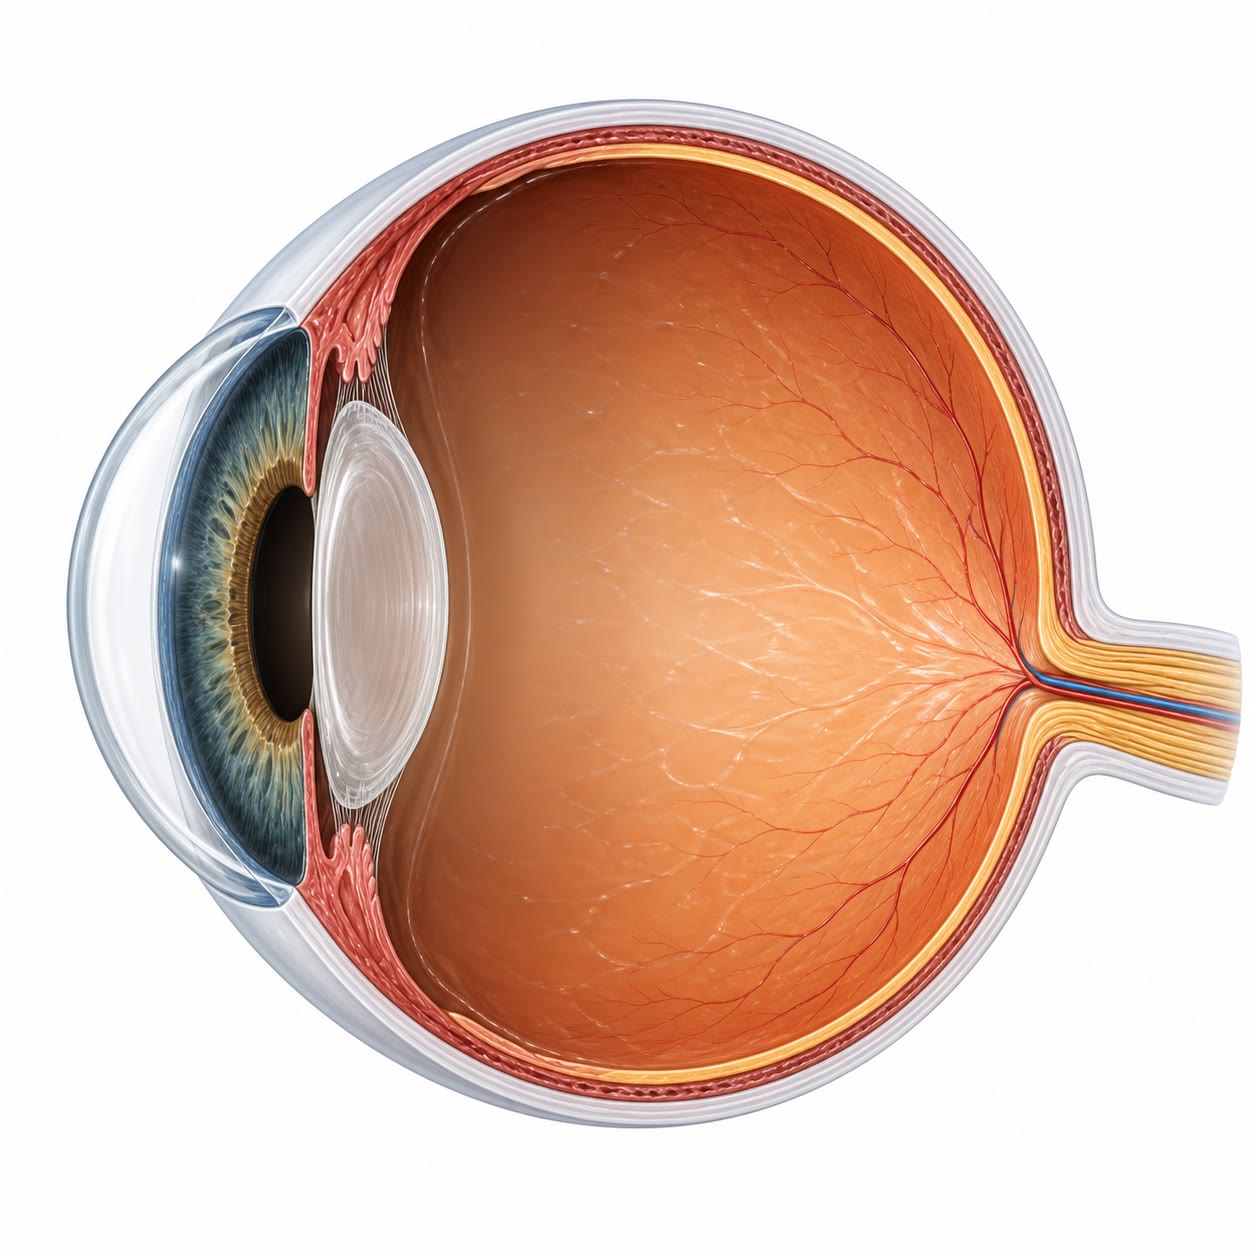
\includegraphics[width=0.46\linewidth]{images/book2/ai/fig-eye-cutaway.jpg}};
  \begin{scope}[x={(img.south east)}, y={(img.north west)},
      every node/.style={font=\small}]
    \draw[omDef, thick] (0.10,0.55) -- (-0.05,0.80) node[left] {角膜};
    \draw[omDef, thick] (0.18,0.36) -- (-0.05,0.20) node[left] {虹膜和瞳孔};
    \draw[omDef, thick] (0.26,0.50) -- (-0.05,0.50) node[left] {晶状体};
    \draw[omDef, thick] (0.55,0.50) -- (0.55,-0.06) node[below] {玻璃体};
    \draw[omDef, thick] (0.83,0.76) -- (1.05,0.88) node[right] {视网膜};
    \draw[omDef, thick] (0.95,0.40) -- (1.05,0.20) node[right] {视神经};
  \end{scope}
\end{tikzpicture}

{\small \omterm{def:g11:the-eye:parts}{眼睛}的水平剖面。角膜与晶状体使
光线会聚；位于后部的视网膜将其转换为信号，
经视神经传出。}
\end{omfigure}

\begin{example}[焦点及其缺陷]\label{ex:g11:the-eye:focus}
放松状态下的\omterm{def:g11:the-eye:parts}{眼睛}能使远处物体成像于视网膜上；要在
\qty{25}{cm} 处阅读，晶状体须变凸。眼球稍长的\omterm{def:g11:the-eye:parts}{眼睛}，远处物体的像
落在视网膜前方——即近视，可用
发散透镜矫正；眼球过短，或晶状体因老化而变硬，
近处物体便无法成像——即远视，
可用凸透镜矫正。两种情形下视网膜均完好，
问题出在光学方面，眼镜的作用
在于使像重新落回感受\omterm{def:g10:cells-common-unit:cell}{细胞}所在之处。
\end{example}

\section{视网膜}

\begin{definition}[光感受器]\label{def:g11:the-eye:photoreceptors}
视网膜含有两类\emph{光感受器}\index{光感受器}
\omterm{def:g10:cells-common-unit:cell}{细胞}，按形状命名。\emph{视杆细胞}\index{视杆细胞}，
约 1.2 亿个，对很弱的光十分敏感，但所含色素只有一种，
使人夜间只能看到灰色的明暗。
\emph{视锥细胞}\index{视锥细胞}约有 600 万个，需要较强的光，
共有三类，各含对光谱不同波段最敏感的一种色素，
使人能在白天看见颜色。
每个光感受器都含有一种\emph{感光色素}——一种
\omterm{def:g11:gene-expression:protein}{蛋白质}，即\emph{视蛋白}\index{视蛋白}，其中结合着一个小的
吸光分子，该分子由维生素 A 衍生而来。感光色素
吸收一个光子后形状发生改变，从而引发\omterm{def:g10:cells-common-unit:cell}{细胞}的电反应。
\end{definition}

\begin{omfigure}
\begin{tikzpicture}[font=\small, >=Stealth, line cap=round]
  % layers from front (left) to back (right); light comes from the left
  \draw[->, very thick, omProp] (-1.6,1.2) -- (-0.3,1.2) node[pos=0, above, omProp] {光};
  % ganglion cells
  \foreach \y in {2.4,1.2,0.0} { \draw[thick, fill=omDef!25] (0.4,\y) circle (0.28); \draw[thick, omDef] (0.12,\y) -- (-0.6,\y) -- (-0.6,-1.4); }
  \node[anchor=north, align=center] at (0.4,-0.5) {神经节 \\ 细胞};
  \draw[->, thick, omDef] (-0.6,-1.4) -- (-0.6,-2.0) node[below, align=center] {传至 \\ 视神经};
  % bipolar cells
  \foreach \y in {2.4,1.2,0.0} { \draw[thick, fill=omMeth!25] (2.2,\y) ellipse (0.22 and 0.36); \draw[thick] (0.68,\y) -- (1.98,\y); \draw[thick] (2.42,\y) -- (3.1,\y); }
  \node[anchor=north, align=center] at (2.2,-0.5) {双极 \\ 细胞};
  % photoreceptors: rods (tall rectangles) and cones (triangles)
  \foreach \y in {2.4,0.0} { \draw[thick, fill=gray!30] (3.1,\y-0.18) rectangle (5.0,\y+0.18); \node[font=\scriptsize] at (4.05,\y) {视杆}; }
  \draw[thick, fill=omThm!25] (3.1,1.2-0.22) -- (5.0,1.2-0.08) -- (5.0,1.2+0.08) -- (3.1,1.2+0.22) -- cycle;
  \node[font=\scriptsize] at (4.05,1.2) {视锥};
  \node[anchor=north, align=center] at (4.5,-0.5) {光感受器 \\ （尖端有色素）};
  % pigment epithelium
  \fill[gray!60] (5.2,-0.2) rectangle (5.6,2.8);
  \node[anchor=west, align=left] at (5.7,1.2) {暗色层 \\ 吸收 \\ 杂散光};
  \node[anchor=south, align=center, font=\scriptsize] at (2.6,3.0) {信号自右向左传递，与光线方向相反};
\end{tikzpicture}

{\small 视网膜剖面图。光穿过透明的
神经\omterm{def:g10:cells-common-unit:cell}{细胞}层，到达后部的\omterm{def:g11:the-eye:photoreceptors}{光感受器}，
其吸光的尖端背向光源；信号随后
依次经感受\omterm{def:g10:cells-common-unit:cell}{细胞}、双极\omterm{def:g10:cells-common-unit:cell}{细胞}传至神经节\omterm{def:g10:cells-common-unit:cell}{细胞}，其纤维
构成视神经。}
\end{omfigure}

\begin{proposition}[视网膜的组织结构]\label{prop:g11:the-eye:organisation}
\omterm{def:g11:the-eye:photoreceptors}{光感受器}位于视网膜后部，紧贴一层暗色层；
光须穿过其他各层才能到达它们。感受器的信号
先传至\emph{双极\omterm{def:g10:cells-common-unit:cell}{细胞}}，再传至\emph{神经节\omterm{def:g10:cells-common-unit:cell}{细胞}}，
其长长的纤维约一百万根，汇集成视神经。
分布并不均匀。在\emph{中央凹}（\omterm{def:g11:the-eye:parts}{眼睛}所正对的小型中央
凹陷处）只有\omterm{def:g11:the-eye:photoreceptors}{视锥细胞}，排列紧密，每个\omterm{def:g11:the-eye:photoreceptors}{视锥细胞}
各与一个神经节\omterm{def:g10:cells-common-unit:cell}{细胞}相连，视觉最为敏锐；远离中心处，
\omterm{def:g11:the-eye:photoreceptors}{视杆细胞}占优势，许多\omterm{def:g11:the-eye:photoreceptors}{视杆细胞}共用一个神经节\omterm{def:g10:cells-common-unit:cell}{细胞}，
灵敏度高，但以细节为代价。视神经离开眼球之处
完全没有感受器，即\emph{盲点}。
\end{proposition}
\admitted

\begin{omfigure}
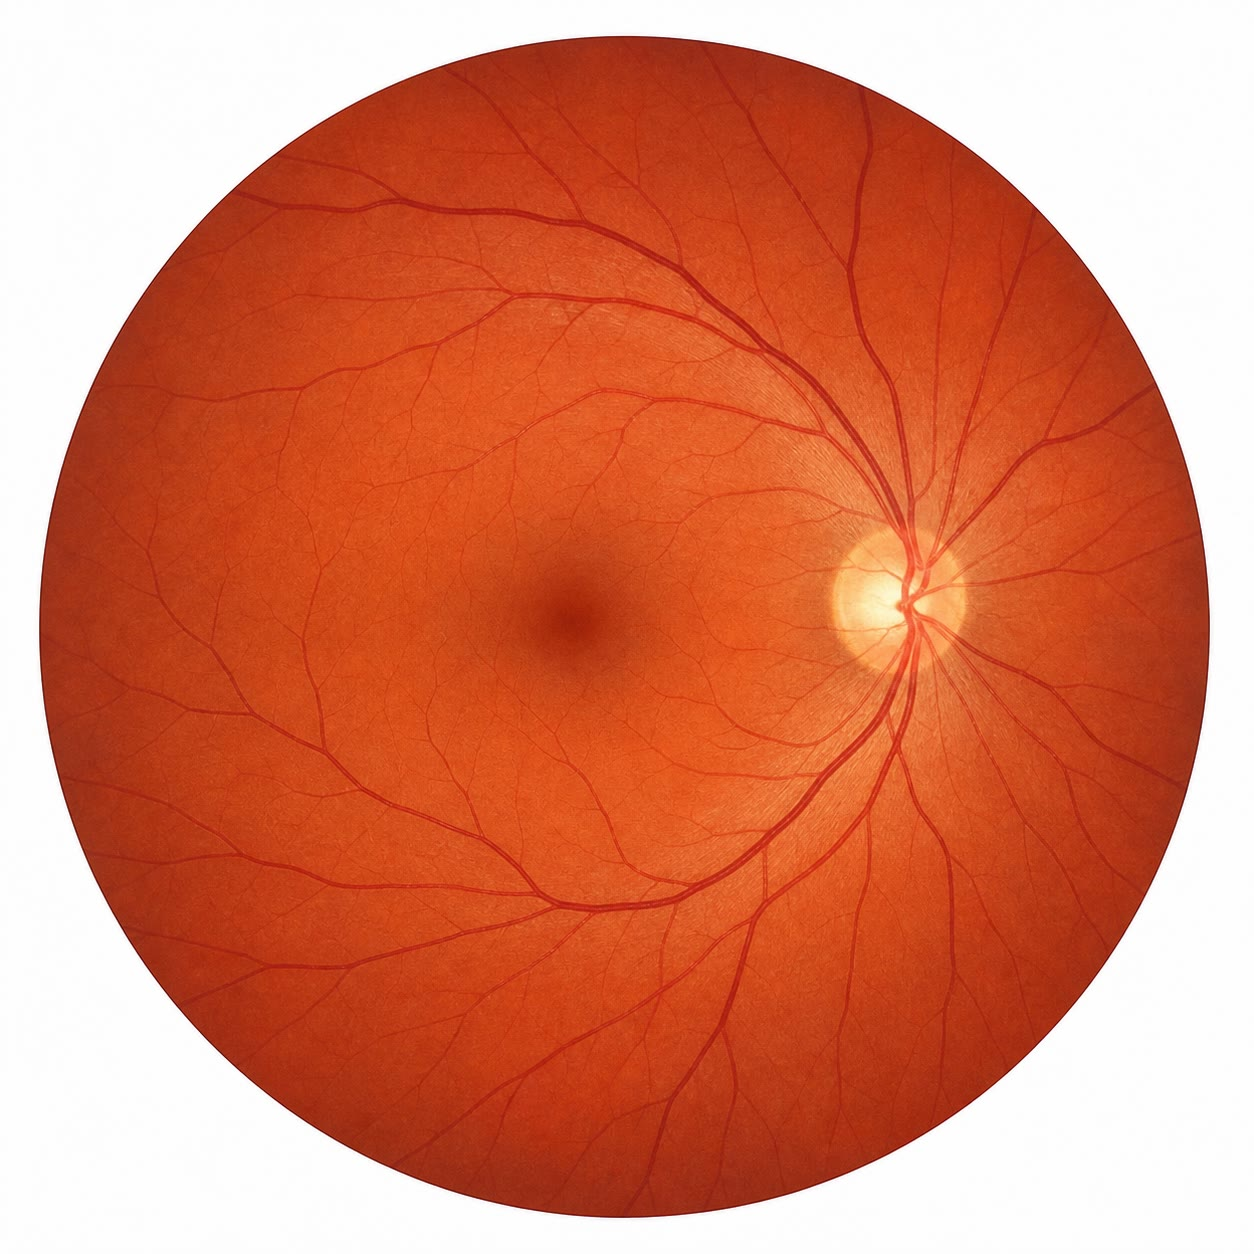
\includegraphics[width=0.42\linewidth]{images/book2/ai/g11-retina-fundus.jpg}

{\small 通过检眼镜经瞳孔所见的视网膜：
视神经离开、血管进入之处为苍白的视盘（即盲点），
另一侧颜色较暗、\omterm{def:g11:the-eye:photoreceptors}{视锥细胞}最密集的是中央凹。}
\end{omfigure}

\begin{example}[两种奇特现象的解释]\label{ex:g11:the-eye:oddities}
直视暗淡的星星时它会消失，因为中央凹只有\omterm{def:g11:the-eye:photoreceptors}{视锥细胞}，
而\omterm{def:g11:the-eye:photoreceptors}{视锥细胞}需要的光比星光所能提供的更多；
斜视时，星光落在\omterm{def:g11:the-eye:photoreceptors}{视杆细胞}上，\omterm{def:g11:the-eye:photoreceptors}{视杆细胞}能探测到它。夜晚外套呈灰色，
是因为看到它的\omterm{def:g11:the-eye:photoreceptors}{视杆细胞}只有一种色素：它们只能报告光的强度，
无法分辨光的波长。颜色是三种\omterm{def:g11:the-eye:photoreceptors}{视锥细胞}之间的比较，
而\omterm{def:g11:the-eye:photoreceptors}{视锥细胞}在黑暗中不工作。
\end{example}

\section{颜色：三种色素}

\begin{proposition}[颜色视觉]\label{prop:g11:the-eye:colour}
每种\omterm{def:g11:the-eye:photoreceptors}{视锥细胞}含有三种\omterm{def:g11:the-eye:photoreceptors}{视蛋白}之一，其吸收峰值分别
位于 \qty{420}{nm}（S 视锥，蓝色）、\qty{530}{nm}（M 视锥，绿色）和
\qty{560}{nm}（L 视锥，红色）附近。某一光线以取决于其波长的比例激活三种\omterm{def:g11:the-eye:photoreceptors}{视锥细胞}，
大脑由这些比例读出颜色。
缺少某一种\omterm{def:g11:the-eye:photoreceptors}{视锥细胞}的人，会混淆该类\omterm{def:g11:the-eye:photoreceptors}{视锥细胞}所能区分的颜色；
若 L 或 M \omterm{def:g11:the-eye:photoreceptors}{视锥细胞}不能正常工作，红色与
绿色便难以分辨——\emph{红绿色盲}，
约 8\% 的男性和 0.5\% 的女性受其影响。
\end{proposition}
\admitted

\begin{omfigure}
\begin{tikzpicture}
\begin{axis}[
  width=0.9\linewidth, height=5.8cm,
  axis x line=bottom, axis y line=left,
  xmin=380, xmax=700, ymin=0, ymax=110,
  xlabel={波长 (nm)}, ylabel={吸收（占峰值的 \%）},
  xlabel style={font=\small, at={(axis description cs:0.5,-0.12)}, anchor=north},
  ylabel style={font=\small},
  tick label style={font=\small}, xtick={400,450,500,550,600,650,700}, ytick={0,50,100},
  legend style={at={(0.5,-0.3)}, anchor=north, legend columns=4, font=\small, draw=none},
]
\addplot[thick, omDef, smooth] coordinates {(380,40) (400,75) (420,100) (440,88) (460,55) (480,25) (500,8) (520,2) (540,0)};
\addplot[thick, gray, dashed, smooth] coordinates {(400,10) (430,35) (460,70) (480,90) (500,100) (520,90) (540,65) (560,38) (580,18) (600,7) (620,2) (640,0)};
\addplot[thick, omMeth, smooth] coordinates {(420,5) (450,20) (480,50) (510,85) (530,100) (550,90) (570,65) (590,38) (610,18) (630,7) (650,2) (670,0)};
\addplot[thick, omThm, smooth] coordinates {(440,5) (470,18) (500,40) (530,80) (560,100) (580,92) (600,70) (620,42) (640,20) (660,8) (680,3) (700,1)};
\legend{S 视锥（蓝）, 视杆, M 视锥（绿）, L 视锥（红）}
\end{axis}
\end{tikzpicture}

{\small 四种光色素的吸收曲线随波长的变化。
各曲线较宽且相互重叠；\qty{580}{nm} 的黄光
强烈激活 L 视锥，中等程度激活 M 视锥，而 S 视锥
完全不被激活——这一比例正是大脑对“黄色”的感知。}
\end{omfigure}

\begin{example}[读取曲线]\label{ex:g11:the-eye:curves}
\qty{500}{nm} 的光：S 视锥为 8\%，M 视锥为 75\%，L 视锥为 40\%——
看起来是蓝绿色。\qty{620}{nm} 的光：S 为 0，M 为 10\%，
L 为 42\%——看起来是红色。缺少 L 视锥的人对两种光只
接收到 S 和 M 的数值，而第二种光给出的 S~0、M~10，
几乎与暗淡的绿色难以区分。缺失的那种\omterm{def:g11:the-eye:photoreceptors}{视锥细胞}
原本能够区分的颜色便合并为一种。
\end{example}

\section{视蛋白基因：一个有历史的基因家族}

\begin{proposition}[视蛋白基因]\label{prop:g11:the-eye:genes}
每种\omterm{def:g11:the-eye:photoreceptors}{视蛋白}由各自的\omterm{def:g10:universal-dna:gene}{基因}编码。S \omterm{def:g11:the-eye:photoreceptors}{视蛋白}\omterm{def:g10:universal-dna:gene}{基因}位于
普通\omterm{def:g11:cell-cycle-mitosis:chromosome}{染色体}上；M 和 L \omterm{def:g11:the-eye:photoreceptors}{视蛋白}\omterm{def:g10:universal-dna:gene}{基因}则并排位于
X \omterm{def:g11:cell-cycle-mitosis:chromosome}{染色体}上。L 与 M 蛋白的 364 个\omterm{def:g10:chemistry-of-life:families}{氨基酸}中，仅有 15 个不同，
（相同度为 96\%），S 蛋白与二者在超过一半的
位置上不同。由于位于 X \omterm{def:g11:cell-cycle-mitosis:chromosome}{染色体}上，一个功能异常的 M 或 L \omterm{def:g10:universal-dna:gene}{等位基因}
会在每个携带它的男性中表达，女性只有携带两份时才会表达——
这正是\cref{ch:g11:genes-and-disease}中的遗传模式，
也解释了为何红绿色盲在男性中的发病率约为女性的十六倍。
\end{proposition}
\admitted

\begin{proposition}[由基因重复产生的基因家族]\label{prop:g11:the-eye:family}
三种\omterm{def:g11:the-eye:photoreceptors}{视蛋白}\omterm{def:g10:universal-dna:gene}{基因}以及视杆色素的\omterm{def:g10:universal-dna:gene}{基因}，都是同一个
祖先\omterm{def:g10:universal-dna:gene}{基因}经\emph{重复}复制而来，随后
又通过\omterm{def:g11:mutations:mutation}{突变}逐渐分化。它们之间的相似程度可用来推断各拷贝产生的时间：S 与
L/M 两支在\omterm{def:g10:common-ancestry:bodyplan}{脊椎动物}历史的很早时期就已分开，距今约 5 亿年；
L 与 M \omterm{def:g10:universal-dna:gene}{基因}来自距今约 3000 万至 4000 万年前
旧世界灵长类祖先中的一次重复，其后代
——猴、猿、人——具有三种\omterm{def:g11:the-eye:photoreceptors}{视锥细胞}，而
大多数其他哺乳动物只有两种。
\end{proposition}
\begin{proof}[证据]
序列比较显示：L 和 M \omterm{def:g10:universal-dna:gene}{基因}相同度为 96\%，并在
X \omterm{def:g11:cell-cycle-mitosis:chromosome}{染色体}上相邻——这是近期串联重复的特征；每个\omterm{def:g10:universal-dna:gene}{基因}与 S \omterm{def:g10:universal-dna:gene}{基因}
约有 43\% 相同，三者与视杆\omterm{def:g11:the-eye:photoreceptors}{视蛋白}\omterm{def:g10:universal-dna:gene}{基因}约有 40\% 相同，
属于较远的拷贝。狗、牛及
大多数哺乳动物在灵长类具有两个\omterm{def:g10:universal-dna:gene}{基因}的位置上只有一个 X 连锁\omterm{def:g11:the-eye:photoreceptors}{视蛋白}\omterm{def:g10:universal-dna:gene}{基因}，
新大陆猴只有一个，且存在若干\omterm{def:g10:universal-dna:gene}{等位基因}，
只有携带两种不同\omterm{def:g10:universal-dna:gene}{等位基因}的雌性才能看到三种颜色。
各谱系中\omterm{def:g10:universal-dna:gene}{基因}数目与\omterm{def:g11:the-eye:photoreceptors}{视锥细胞}种类相符，
\omterm{def:g10:universal-dna:gene}{基因}树与\omterm{def:g10:biodiversity-scales:species}{物种}树也相互吻合。
\end{proof}

\begin{omfigure}
\begin{tikzpicture}[font=\small, line cap=round]
  % gene tree: root -> (rod opsin) ; (S) ; (L/M split)
  \draw[thick] (0,2) -- (1.5,2);
  \draw[thick] (1.5,2) -- (1.5,3.4) -- (9,3.4);
  \draw[thick] (1.5,2) -- (1.5,0.6) -- (3.2,0.6);
  \draw[thick] (3.2,0.6) -- (3.2,1.8) -- (9,1.8);
  \draw[thick] (3.2,0.6) -- (3.2,-0.6) -- (7.6,-0.6);
  \draw[thick] (7.6,-0.6) -- (7.6,0.2) -- (9,0.2);
  \draw[thick] (7.6,-0.6) -- (7.6,-1.4) -- (9,-1.4);
  \fill[omThm] (1.5,2) circle (2.5pt); \fill[omThm] (3.2,0.6) circle (2.5pt); \fill[omThm] (7.6,-0.6) circle (2.5pt);
  \node[anchor=west] at (9.1,3.4) {视杆视蛋白（视紫红质）};
  \node[anchor=west] at (9.1,1.8) {S 视蛋白（蓝色视锥）};
  \node[anchor=west] at (9.1,0.2) {M 视蛋白（绿色视锥）};
  \node[anchor=west] at (9.1,-1.4) {L 视蛋白（红色视锥）};
  \node[anchor=south, font=\scriptsize, omThm] at (1.5,3.5) {很早时的重复};
  \node[anchor=north, font=\scriptsize, omThm, align=center] at (3.2,-0.75) {重复 \\ $\sim$5 亿年前};
  \node[anchor=north, font=\scriptsize, omThm, align=center] at (7.6,-1.55) {重复 \\ $\sim$3500 万年前};
  \node[anchor=east] at (-0.1,2) {祖先视蛋白基因};
  \draw[->, gray] (0,-2.3) -- (9,-2.3) node[midway, below, font=\scriptsize] {时间};
\end{tikzpicture}

{\small \omterm{def:g11:the-eye:photoreceptors}{视蛋白}\omterm{def:g10:universal-dna:gene}{基因}家族。每个红点代表一次重复：一个\omterm{def:g10:universal-dna:gene}{基因}变成两个，
之后两个拷贝各自因\omterm{def:g11:mutations:mutation}{突变}而分化。最近的一次
是 L/M 重复，仅见于旧大陆灵长类，使它们多出第三种视锥。}
\end{omfigure}

\begin{example}[一次重复改变了什么]\label{ex:g11:the-eye:duplication}
只有两种视锥的猴子看到的森林，颜色只有两个维度，
成熟的果实很难从叶丛中分辨出来。L/M
重复之后，其中一个拷贝可以向更长的波长\omterm{def:g11:mutations:mutation}{突变}，而
另一个保留原样——于是出现了第三种视锥，成熟的红色果实便能与
绿色叶丛区分开。之后使约 8\% 男性一个拷贝失效的\omterm{def:g11:mutations:mutation}{突变}，只是
让\omterm{def:g11:the-eye:parts}{眼睛}回到祖先的两种视锥状态。
\end{example}

\begin{method}[色觉案例的推理]\label{met:g11:the-eye:case}
\begin{enumerate}
  \item 缺失或改变的是哪一种视锥？从
        所混淆的颜色判断：红–绿混淆为 L 或 M；蓝–黄混淆（罕见）为 S。
  \item 是哪个\omterm{def:g10:universal-dna:gene}{基因}，位于哪条\omterm{def:g11:cell-cycle-mitosis:chromosome}{染色体}上？L 和 M 位于 X \omterm{def:g11:cell-cycle-mitosis:chromosome}{染色体}，S
        位于其他\omterm{def:g11:cell-cycle-mitosis:chromosome}{染色体}。
  \item 运用遗传规律：红–绿色盲为 X 连锁\omterm{def:g11:genes-and-disease:genetic}{隐性}遗传——
        携带者母亲所生的儿子有一半患病，患病父亲所生的女儿
        全部是携带者。
  \item 与\omterm{def:g10:universal-dna:gene}{基因}家族相联系：一个拷贝丢失，或 L 和 M
        拷贝因相邻\omterm{def:g10:universal-dna:gene}{基因}之间的交换而变得过于相似。
\end{enumerate}
\end{method}

\begin{remark}[从眼睛到大脑]\label{rem:g11:the-eye:tobrain}
视网膜并不“看”；它进行转换，并开始分类。视神经中约一百万根纤维
把经过编码的描述——对比度、
边缘、视锥反应的比值——传送到大脑，由下一章接手处理。
我们所说的看见，正是在那里形成的，
它只依赖于这里所述\omterm{def:g10:cells-common-unit:cell}{细胞}的信号，别无其他：视网膜正常而视觉脑受损的人，
是盲的；而
视觉脑正常但\omterm{def:g11:the-eye:photoreceptors}{光感受器}已死亡的人，
同样是盲的。
\end{remark}

\section{练习}

\begin{exercise}[$\star$]\label{exo:g11:the-eye:1}
按顺序列出光从外界到达
\omterm{def:g11:the-eye:photoreceptors}{光感受器}所经过的结构。
\end{exercise}

\begin{exercise}[$\star$]\label{exo:g11:the-eye:2}
比较\omterm{def:g11:the-eye:photoreceptors}{视杆细胞}与\omterm{def:g11:the-eye:photoreceptors}{视锥细胞}：数量、灵敏度、色素、视觉类型。
\end{exercise}

\begin{exercise}[$\star$]\label{exo:g11:the-eye:3}
什么是中央凹和盲点？
\end{exercise}

\begin{exercise}[$\star$]\label{exo:g11:the-eye:4}
根据吸收光谱图，哪些色素吸收
\qty{450}{nm} 的光，吸收强度如何？
\end{exercise}

\begin{exercise}[$\star$]\label{exo:g11:the-eye:5}
L 和 M \omterm{def:g11:the-eye:photoreceptors}{视蛋白}\omterm{def:g10:universal-dna:gene}{基因}位于哪条\omterm{def:g11:cell-cycle-mitosis:chromosome}{染色体}上？这对
红–绿色盲的遗传有何影响？
\end{exercise}

\begin{exercise}[$\star\star$]\label{exo:g11:the-eye:6}
解释为什么夜晚看不到颜色，以及为什么较暗的恒星
用斜视更容易看清。
\end{exercise}

\begin{exercise}[$\star\star$]\label{exo:g11:the-eye:7}
两束光对视锥的刺激如下：光 1，S 为 0，M 为 60，L 为 100；
光 2，S 为 0，M 为 30，L 为 50。它们颜色相同吗？亮度
是否相同？请说明理由。
\end{exercise}

\begin{exercise}[$\star\star$]\label{exo:g11:the-eye:8}
一名色盲男性与一名家族中没有色盲成员的女性结婚。
求他们的儿子、女儿，以及
女儿之子的颜色视觉情况。
\end{exercise}

\begin{exercise}[$\star\star$]\label{exo:g11:the-eye:9}
为什么红–绿色盲在男性中的发病率是女性的十六倍？
由男性中的 8\% 计算女性中的预期频率。
\end{exercise}

\begin{exercise}[$\star\star$]\label{exo:g11:the-eye:10}
L 与 M \omterm{def:g10:universal-dna:gene}{基因}序列相同率为 96\%，二者各与 S \omterm{def:g10:universal-dna:gene}{基因}序列相同 43\%。
解释这两个数值如何说明各次重复之间的
先后关系。
\end{exercise}

\begin{exercise}[$\star\star$]\label{exo:g11:the-eye:11}
大多数哺乳动物有两种视锥，旧大陆灵长类有三种。用一次重复解释
这一差异，并说明为什么这一变化可能被保留。
\end{exercise}

\begin{exercise}[$\star\star\star$]\label{exo:g11:the-eye:12}
某人缺少 S 视锥。他会混淆哪些颜色？解释
为什么这种情况罕见，且在两性中的发生频率相同。
\end{exercise}

\begin{exercise}[$\star\star\star$]\label{exo:g11:the-eye:13}
中央凹处的视锥相距 \qty{2.5}{\micro m}，\omterm{def:g11:the-eye:parts}{眼睛}的焦距
约为 \qty{17}{mm}。计算两点仍能落在不同视锥上的
最小张角，以及
在 \qty{10}{m} 处可分辨的最小细节的大小。（使用小角度近似：
弧度制角度 $=$ 大小 $/$ 距离。）
\end{exercise}

\begin{exercise}[$\star\star\star$]\label{exo:g11:the-eye:14}
在新世界猴中，单个 X 连锁的\omterm{def:g11:the-eye:photoreceptors}{视蛋白}\omterm{def:g10:universal-dna:gene}{基因}有若干
不同峰值波长的\omterm{def:g10:universal-dna:gene}{等位基因}。解释为何只有部分\omterm{def:g10:biodiversity-scales:species}{物种}的雌性
能看到三种颜色，而雄性均不能。
\end{exercise}

\begin{exercise}[$\star\star\star$]\label{exo:g11:the-eye:15}
某种疾病破坏了\omterm{def:g11:the-eye:photoreceptors}{光感受器}，而视网膜的其余部分
未受损。解释为何以电刺激神经节\omterm{def:g10:cells-common-unit:cell}{细胞}的植入装置
能够恢复部分视力，并说明其视觉质量受何限制。
\end{exercise}

\section{问题：三种色素与一次基因重复}

\begin{problem}[{周末问题——拆解色觉：光谱上的视锥响应、
一个色盲家族、视蛋白基因的比较，
以及中央凹能达到的清晰度}]
\label{pb:g11:the-eye:1}
请利用吸收图。一项测试给出了波长为 \qty{470}{nm}、
\qty{530}{nm}、\qty{590}{nm} 和 \qty{650}{nm} 的光。

\medskip
\noindent\textbf{第一部分——视锥作出响应。}
\begin{enumerate}
  \item 对每种光，读取 S、M 和
        L 视锥的近似响应。
  \item 哪种光能同时激发三种视锥？哪种光只能激发一种？
  \item 缺少 L 视锥的人只接收 S 和 M 的数值。
        四种光中，哪两种对他难以区分？
        请结合数值说明理由。
  \item 缺少 M 视锥的人：她会混淆哪一对？
  \item 解释为何两人都不是“对红色失明”，但都
        难以分辨红色与绿色。
\end{enumerate}

\medskip
\noindent\textbf{第二部分——一个家族。}
诺拉色觉正常；她的父亲患红绿色盲。她
与色觉正常的萨姆结婚。
\begin{enumerate}[resume]
  \item 写出诺拉在 X 连锁\omterm{def:g11:the-eye:photoreceptors}{视蛋白}\omterm{def:g10:universal-dna:gene}{基因}上的\omterm{def:g11:enzymes-and-phenotype:phenotype}{基因型}，并说明理由。
  \item 写出他们可能的儿子和女儿的\omterm{def:g11:enzymes-and-phenotype:phenotype}{基因型}与色觉，
        并给出相应概率。
  \item 他们色觉正常的女儿伊内丝，与一名
        色盲男性结婚。求伊内丝是携带者的概率，
        再求他们的一个女儿是色盲的
        概率。
  \item 解释为何色盲的女儿，其父亲
        必然也是色盲。
  \item 诺拉父亲的母亲色觉正常。她一定是
        携带者吗？请说明理由。
\end{enumerate}

\medskip
\noindent\textbf{第三部分——\omterm{def:g10:universal-dna:gene}{基因}。}
\omterm{def:g11:the-eye:photoreceptors}{视蛋白}序列之间的同一性：L--M 96\%，L--S 43\%，M--S
43\%，S--视紫红质 41\%。
\begin{enumerate}[resume]
  \item 画出或描述由这些数值推断出的四个\omterm{def:g10:universal-dna:gene}{基因}的
        系统发生树。
  \item 若差异以稳定速率积累，且 L/M \omterm{def:g10:universal-dna:gene}{基因}重复
        发生于 35 百万年前，估算 S 与 L/M 分化
        的年代。
  \item L 与 M \omterm{def:g10:universal-dna:gene}{基因}在 X \omterm{def:g11:cell-cycle-mitosis:chromosome}{染色体}上彼此相邻。解释减数分裂中二者之间的
        不等交换如何产生只携带两者之一的 X \omterm{def:g11:cell-cycle-mitosis:chromosome}{染色体}，
        以及由此产生怎样的色觉。
  \item 此类交换是红绿色盲最常见的原因。为何两个
        相邻且几乎相同的\omterm{def:g10:universal-dna:gene}{基因}
        特别容易发生此类交换？
  \item L/M 重复存在于所有旧大陆灵长类中，而在
        其他哺乳动物中并不存在。这说明该重复发生于何时、
        发生于哪些生物之中？
\end{enumerate}

\medskip
\noindent\textbf{第四部分——中央凹的清晰度。}
中央凹视锥之间相距 \qty{2.5}{\micro m}；\omterm{def:g11:the-eye:parts}{眼睛}的焦距
为 \qty{17}{mm}。使用张角（以弧度计）$=$ 大小 $/$ 距离。
\begin{enumerate}[resume]
  \item 计算两相邻视锥所张的角，分别以弧度和
        角分表示（$1' = \num{2.9e-4}$ rad）。
  \item 在 \qty{6}{m} 处能分辨的最小字母细节有多大？
        请与视力表上字母的笔画作比较，
        该距离下“正常”视力的笔画约为 \qty{1.7}{mm}。
  \item 远离中央凹处，100 个\omterm{def:g11:the-eye:photoreceptors}{视杆细胞}共用一个
        神经节\omterm{def:g10:cells-common-unit:cell}{细胞}。估算此处可分辨的张角，并说明
        这样换来了什么。
  \item 鹰的中央凹视锥密度是两倍，且其\omterm{def:g11:the-eye:parts}{眼睛}
        略大。其分辨率较人眼提高了多少倍？
  \item 归纳结论：三种视锥类型及各自不敏感的光，
        使灵长类获得第三种视锥的单一遗传事件，
        以及中央凹所能分辨的张角。
\end{enumerate}
\end{problem}
